% Copyright (c) 2015 Benito Palacios Sánchez - All Rights Reserved.
% Esta obra está licenciada bajo la Licencia Creative Commons Atribución 4.0
% Internacional. Para ver una copia de esta licencia, visita
% http://creativecommons.org/licenses/by/4.0/.

% Template
\documentclass[usenames,dvipsnames]{beamer}
\pdfoutput=1

% Notes. Uncomment to view the notes.
%\setbeameroption{show notes}
%\setbeamertemplate{note page}[plain]    % Remove the note page style

% Load this package to allow load many big packages.
\usepackage{etex}

% Font
\usepackage[T1]{fontenc}        % Output font
\usepackage[utf8]{inputenc}     % Input encoding
\usepackage[spanish]{babel}     % For Spanish texts
\usepackage{FiraSans}           % For FiraSans beauty fonts

% Theme
\usetheme{Darmstadt}
\usecolortheme{whale}

% Other packages
\usepackage{xcolor}             % For color in text
\usepackage{url}                % For links
\usepackage{pifont}             % For tick symbol
\usepackage{graphicx}           % For graphics
\usepackage{epstopdf}           % For EPS graphics in Windows
\usepackage{multimedia}         % For media
\usepackage{ctable}             % For tables
\usepackage{verbatim}           % For non-parsed text blocks
\usepackage{tikz}               % To draw over images
\usepackage{textcomp}           % For text arrows.
\usepackage{listings}           % For blocks of code
\lstset{language=[Sharp]C,basicstyle=\scriptsize\ttfamily, keywordstyle=\scriptsize\color{blue}\ttfamily}

% My package
\usepackage{../Layout}

% Information about author and document
\title{Introducción al ROM Hacking}
\subtitle{Primeros pasos}
\date[Marzo de 2016]{30 de marzo de 2016}
\author{Benito Palacios Sánchez}
\authortitle{}
\authoremail{benito.palaciossanchez.es@ieee.org}
\institute[IEEE SB UGR]{Rama estudiantil de IEEE en la UGR}
\titlelogo{../logo.png}

% Add a little logo in the corner of the slides
\pgfdeclareimage[height=0.5cm]{logo-mini}{../logo_mini.png}
\logo{\pgfuseimage{logo-mini}}

\begin{document}

    % Title page
    {
    \usebackgroundtemplate{
        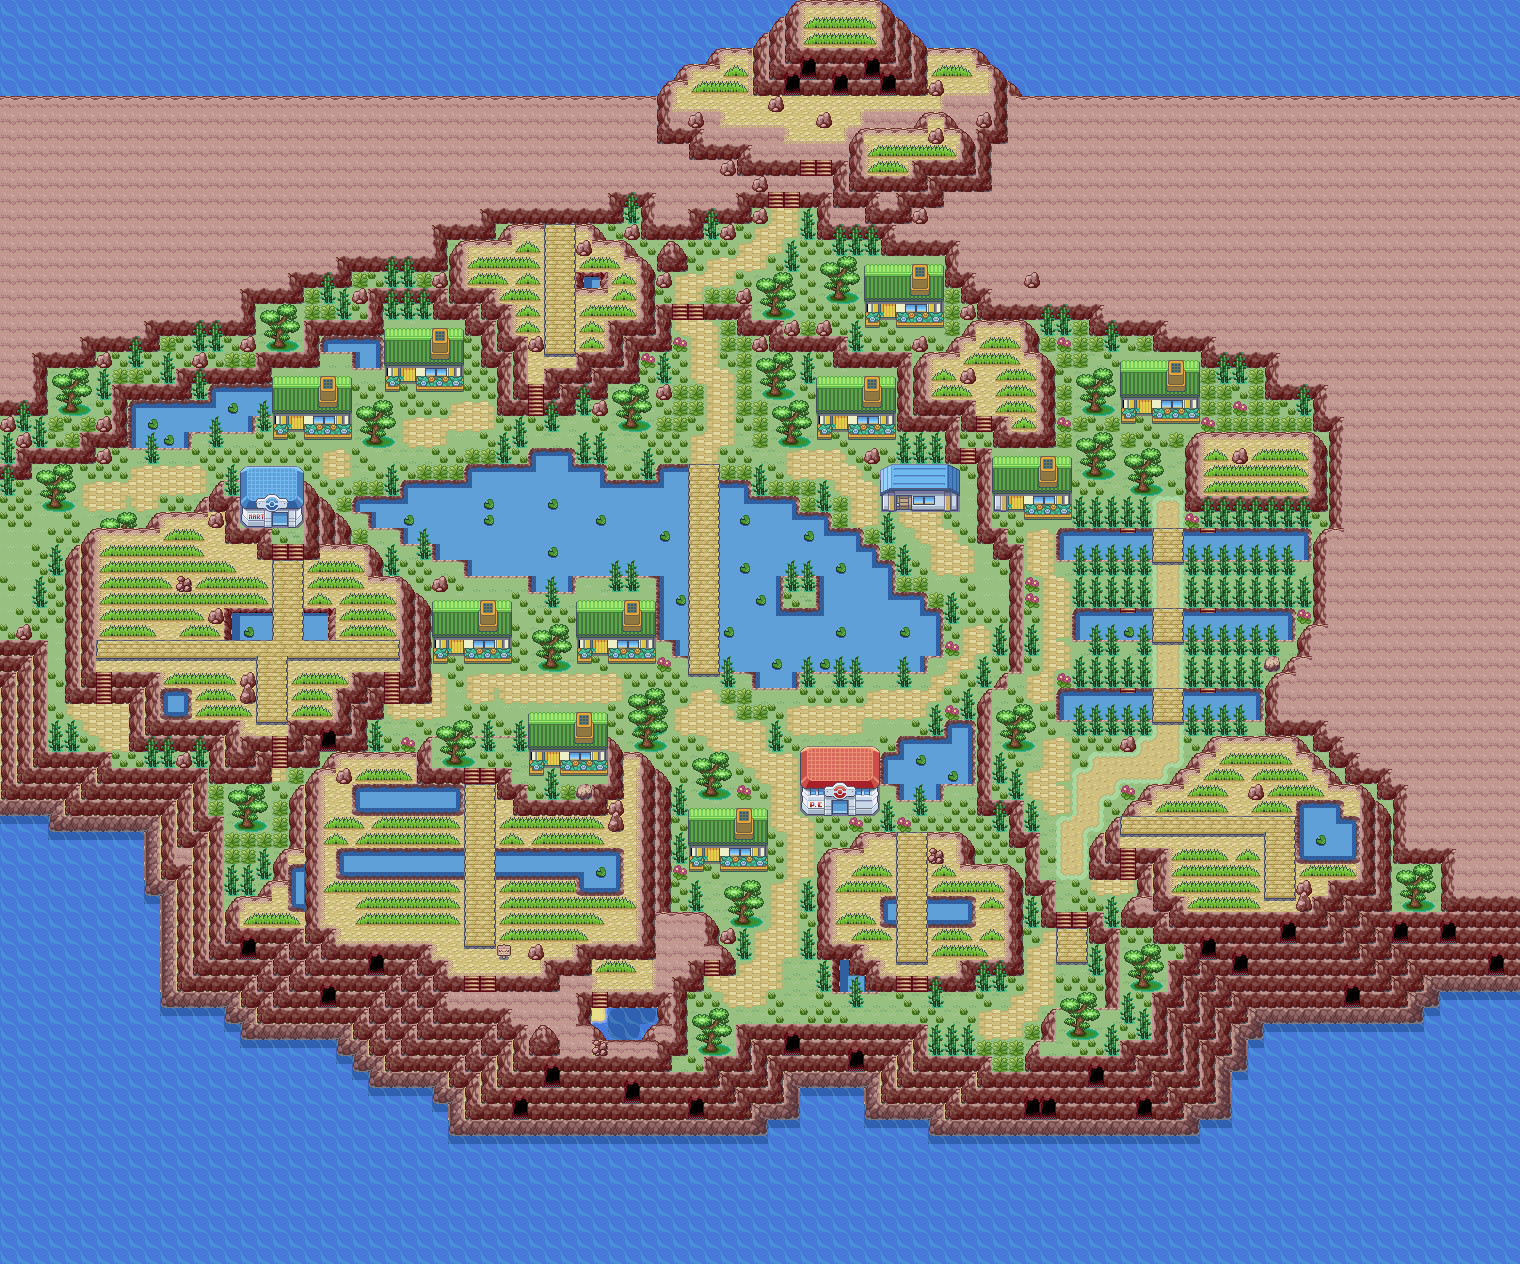
\includegraphics[width=\paperwidth]{imgs/bg_hack.jpg}}
    \begin{frame}[plain]
        \titlepage{}
    \end{frame}
    }

    % Content
    \section{Introducción}
\subsection{Sobre mi\ldots}
\begin{frame}{¿Quién soy?}

    \begin{columns}
    \begin{column}{0.75\textwidth}
        \Large
        Benito Palacios Sánchez \\
        \textbf{@pleonex}
    \end{column}
    \begin{column}{0.25\textwidth}
        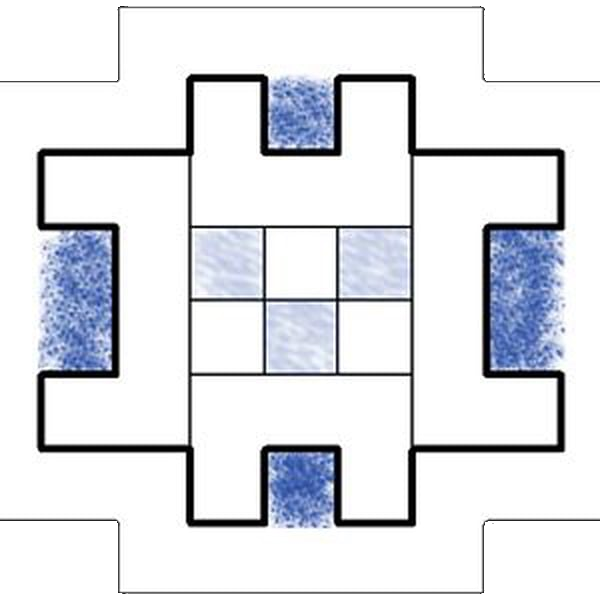
\includegraphics[width=\textwidth]{imgs/pleonex.png}
    \end{column}
    \end{columns}

    \vfill
    \setlength{\leftmargini}{0em}
    \begin{itemize}
        \item<2-> Graduado en Ingeniería de Tecnologías de Telecomunicación
        \begin{itemize}
            \item <2-> Trabajo Fin de Grado sobre seguridad en videojuegos
        \end{itemize}
        \item<3-> Miembro de IEEE Student Branch of Granada
        \item<4-> \textgreater 6 años en el mundo del ROM Hacking
        \item<5-> Miembro de GradienWords
    \end{itemize}
\end{frame}

\begin{frame}{Mis proyectos}
    \setlength{\leftmargini}{0em}
    \begin{columns}
    \begin{column}[T]{0.5\textwidth}
        \large \centering
        Tinke
        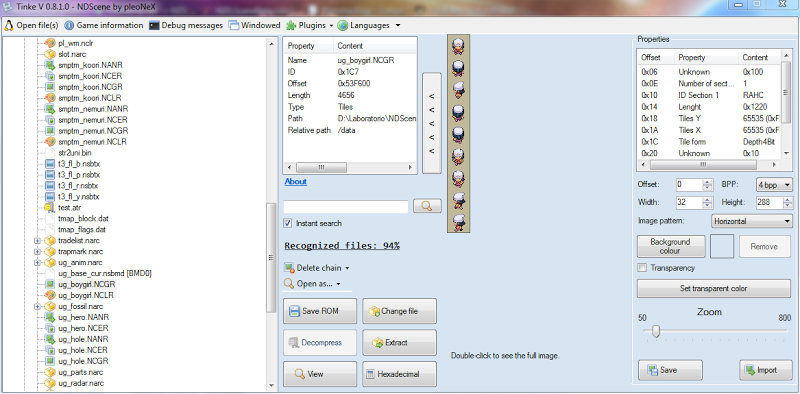
\includegraphics[width=\textwidth]{imgs/tinke_preview.png}
    \end{column}
    \begin{column}[T]{0.65\textwidth}
        \large \centering
        \uncover<2->{Ninokuni: El Mago de las Tinieblas}
        \visible<2->{\includegraphics[width=0.5\textwidth]{imgs/ninokuni_preview.jpg}}
    \end{column}
    \end{columns}

    \vfill
    \small
    \begin{columns}
    \begin{column}{0.3\textwidth}
        \uncover<3->{NinoDrive \\}
        \uncover<3->{NinoImager \\}
        \uncover<3->{NinoDecompiler}
    \end{column}
    \begin{column}{0.3\textwidth}
        \uncover<3->{NinoPatcher \\}
        \uncover<3->{Zerum \\}
        \uncover<3->{NerdFontTerminatoR}
    \end{column}
    \begin{column}{0.3\textwidth}
        \uncover<3->{Modime \\}
        \uncover<3->{NitroDebugger \\}
        \uncover<3->{Sadler}
    \end{column}
    \end{columns}

    \vfill
    \begin{columns}
    \begin{column}{0.5\textwidth}
        \uncover<4->{Final Fantasy: Four Heroes \\}
        \uncover<4->{Blood of Bahamut \\}
        \uncover<4->{Profesor Layton: London Life \\}
        \uncover<4->{Ace Attorney Investigation 2}
    \end{column}
    \begin{column}{0.5\textwidth}
        \uncover<4->{Shining Force Feather \\}
        \uncover<4->{Pokémon Conquest \\}
        \uncover<4->{Inazuma Eleven 2 \\}
        \uncover<4->{Resident Evil 2}
    \end{column}
    \end{columns}
\end{frame}

\subsection{El Big Bang}
\begin{frame}{Érase una vez\ldots}
    \visible<2->{\centering 
\includegraphics[width=0.65\textwidth]{imgs/bigbang.png}}
\end{frame}

\begin{frame}{¿Qué es un fichero?}
    \centering\fontsize{80}{0}\selectfont
    ¿ \includegraphics{imgs/file.png}~?
    \note<1>{Un fichero es simplemente un conjunto de bytes con significado.}
\end{frame}

\begin{frame}[t]{¿Qué hay dentro de un fichero?}
    \huge\centering
    \uncover<2->{¿Qué hay para que veamos\ldots \\}
    \uncover<3->{\ldots imágenes? \\}
    \uncover<4->{\ldots vídeos? \\}
    \uncover<5->{\ldots música? \\}
    \vfill
    \uncover<6->{¿Cómo lo vemos eso?}
\end{frame}

\begin{frame}{La parte cruda de los archivos}
    \includefigure{BMP visto con editor hexadecimal HxD}{imgs/hexview.png}{0.6}
\end{frame}

\begin{frame}[fragile]{Especificaciones (BMP)}
    \footnotesize
    \ctable[]{ccl}{}{                                                       \FL
        Posición      & Tamaño        & Descripción                         \ML
        \multicolumn{3}{c}{Cabecera estándar}                               \NN
        \texttt{0x00} & \texttt{0x02} & \textit{Magic stamp}: \texttt{BM}   \NN
        \texttt{0x02} & \texttt{0x04} & Tamaño del fichero                  \NN
        \texttt{0x06} & \texttt{0x04} & Reservado                           \NN
        \texttt{0x0A} & \texttt{0x04} & Puntero a los datos de la imagen    \ML
        \multicolumn{3}{c}{Cabecera DIB}                                    \NN
        \texttt{0x00} & \texttt{0x04} & Tamaño de esta cabecera             \NN
        \texttt{0x04} & \texttt{0x04} & Ancho de la imagen                  \NN
        \texttt{0x06} & \texttt{0x04} & Alto de la imagen                   \NN
        \texttt{0x08} & \texttt{0x02} & Número de planos de color (1)       \NN
        \texttt{0x0A} & \texttt{0x02} & Número de bits por píxel            \ML
        \multicolumn{3}{c}{Paleta de colores}                               \ML
        \multicolumn{3}{c}{Píxeles}                                         \LL
    }
\end{frame}

\begin{frame}{Especificaciones (BMP)}
    \begin{columns}
    \begin{column}[T]{0.7\textwidth}
        \begin{tikzpicture}
        \node[anchor=south west,inner sep=0] (image) at (0,0)
        {\includegraphics[width=\textwidth]{imgs/hexview.png}};
            \begin{scope}[x={(image.south east)},y={(image.north west)}]
                \draw<1,6->[red,semithick] (0.15,0.785) rectangle (0.64,0.76);
                \draw<2-5>[red,semithick] (0.15,0.76) rectangle (0.22,0.785);
                \draw<3-5>[red,semithick] (0.22,0.76) rectangle (0.36,0.785);
                \draw<4-5>[red,semithick] (0.36,0.76) rectangle (0.50,0.785);
                \draw<5>[red,semithick] (0.50,0.76) rectangle (0.64,0.785);
                \draw<6,13->[green,semithick] (0.64,0.76) -- (0.64,0.785) -- (0.72,0.785) -- (0.72,0.605) -- (0.50,0.605) -- (0.50,0.58) -- (0.15,0.58) -- (0.15,0.76) -- (0.64,0.76);
                \draw<7-12>[green,semithick] (0.72,0.76) -- (0.64,0.76) -- (0.64,0.785) -- (0.72,0.785);
                \draw<7-12>[green,semithick] (0.15,0.76) -- (0.22,0.76) -- (0.22,0.735) -- (0.15,0.735);
                \draw<8-12>[green,semithick] (0.22,0.735) rectangle (0.36,0.76);
                \draw<9-12>[green,semithick] (0.36,0.735) rectangle (0.50,0.76);
                \draw<10-12>[green,semithick] (0.50,0.735) rectangle (0.57,0.76);
                \draw<11-12>[green,semithick] (0.57,0.735) rectangle (0.64,0.76);
                \draw<12>[green,semithick] (0.64,0.735) -- (0.64,0.76) -- (0.72,0.76) -- (0.72,0.605) -- (0.50,0.605) -- (0.50,0.58) -- (0.15,0.58) -- (0.15,0.735) -- (0.64,0.735);
                \draw<13->[blue,semithick] (0.15,0.12) -- (0.15,0.58) -- (0.50,0.58) -- (0.50,0.605) -- (0.72,0.605) -- (0.72, 0.145) -- (0.50,0.145) -- (0.50,0.12) -- (0.15,0.12);
                \draw<14->[black,semithick] (0.15,0.04) -- (0.15,0.12) -- (0.50,0.12) -- (0.50,0.145) -- (0.72,0.145) -- (0.72,0.04) ;
            \end{scope}
        \end{tikzpicture}
    \end{column}
    \hfill
    \begin{column}[T]{0.4\textwidth}
        \begin{enumerate}
            \item<1-> Cabecera estándar
            \begin{enumerate}
                \item<2-> \textit{Magic stamp}
                \item<3-> Tamaño fichero
                \item<4-> Reservado
                \item<5-> Puntero datos
            \end{enumerate}
            \item<6-> Cabecera DIB
            \begin{enumerate}
                \item<7-> Tamaño DIB
                \item<8-> Ancho
                \item<9-> Alto
                \item<10-> Planos de color
                \item<11-> BPP
                \item<12-> Meta-datos
            \end{enumerate}
            \item<13-> Paleta
            \item<14-> Píxeles
        \end{enumerate}
    \end{column}
    \end{columns}
\end{frame}

\begin{frame}{¿Qué hay dentro de un juego?}
    \fontsize{45}{0}\selectfont
    \begin{columns}
    \begin{column}{0.65\textwidth}
        ¿ \includegraphics{imgs/gamefile.png}~?
        \visible<2->{\textrightarrow}
    \end{column}
    \hfill
    \begin{column}{0.35\textwidth}
        \visible<2->{\includegraphics[width=\textwidth]{imgs/game_desmume.png}}
    \end{column}
    \end{columns}
\end{frame}

\begin{frame}{La parte cruda de un juego}
    \includegraphics[width=\textwidth]{imgs/game_hex.png}
\end{frame}

\begin{frame}{¿Y ahora? ¿Y la especificación?}
    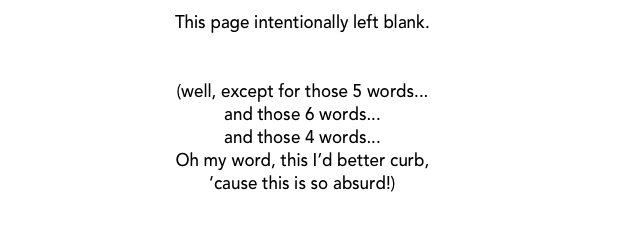
\includegraphics[width=\textwidth]{imgs/left_blank.png}
\end{frame}

\begin{frame}{ROM Hacking}
    \includegraphics[width=\textwidth]{imgs/this_is_romhacking.png}
\end{frame}

\begin{frame}{ROM Hacking}
    \begin{columns}
    \begin{column}{0.35\textwidth}
        Propósito:
        \begin{itemize}
            \item<2-> Fan traducciones
            \item<3-> Mods
            \item<4-> Extraer recursos
            \item<5-> Curiosidad
        \end{itemize}
    \end{column}
    \begin{column}{0.65\textwidth}
        \centering
        \visible<2->{\includegraphics[width=0.45\textwidth]{imgs/ninokuni_preview.jpg}}
        \visible<3->{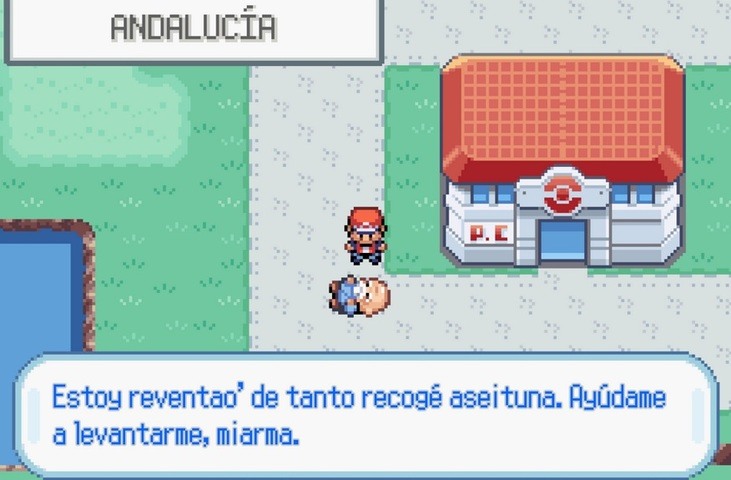
\includegraphics[width=0.45\textwidth]{imgs/mods_preview.jpg}}
        \visible<4->{\includegraphics[width=0.4\textwidth]{imgs/spriters.png}}
        \visible<5->{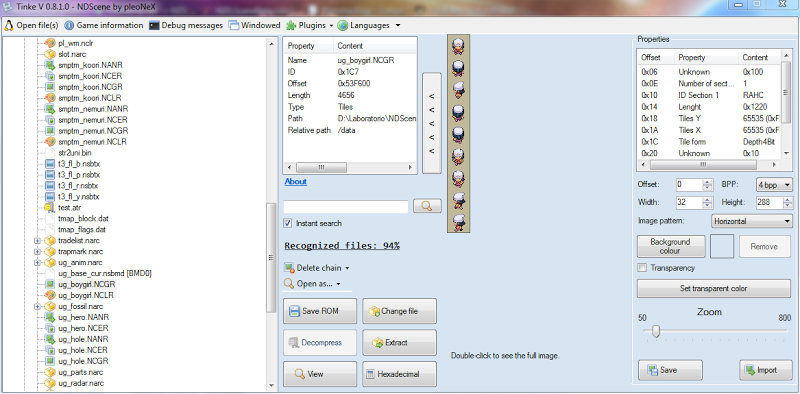
\includegraphics[width=0.8\textwidth]{imgs/tinke_preview.png}}
    \end{column}
    \end{columns}
\end{frame}

\subsection{Temario}
\begin{frame}<beamer:0|handout:0>{Contenido del curso}
    \centering
    \textbf{Introducción al ROM Hacking}
    \begin{enumerate}
        \item<+-> Edita tu primer videojuego
        \begin{enumerate}
            \item ¿Qué es ROM Hacking?
            \item Modifica un videojuego
        \end{enumerate}
        \item<+-> Formatos estándar en Nintendo DS
        \begin{enumerate}
            \item Textos y tipografías
            \item Compresiones
            \item Imágenes y modelos 3D
            \item Audios
        \end{enumerate}
        \item<+-> Programas de edición de ficheros
        \begin{enumerate}
            \item Crystal Tile
            \item New Super Mario Bros Level Editor
            \item Super Mario 64 DS Editor
            \item Pokémon
            \item Ninokuni
            \note<1>{TileMolester, DSLazy, CUE Compressors}
        \end{enumerate}
    \end{enumerate}
\end{frame}

\begin{frame}<beamer:0|handout:0>{Futuros cursos}
    \begin{columns}
    \begin{column}{0.5\textwidth}
        \uncover<2->{\textbf{Desarrollo de herramientas de ROM Hacking}
        \begin{enumerate}
            \item Crear plugins para Tinke y Libgame.
            \item Crear programas editores de script, imágenes, \ldots
        \end{enumerate}}
    \end{column}
    \hfill
    \begin{column}{0.5\textwidth}
        \uncover<3->{\textbf{ROM Hacking sobre ensamblador}
        \begin{enumerate}
            \item Aprender ensamblador
            \item Depurar juegos
            \item Modificar el código fuente de juegos
        \end{enumerate}}
    \end{column}
    \end{columns}
\end{frame}

    \section{Hello World!}
\begin{frame}{Hello World!}
    \Huge\centering\textbf{ROM HACKING TIME!}
\end{frame}

\subsection{NitroROM}
\begin{frame}{Especificación de juegos de NDS}
    \begin{block}{GBATEK}
        \centering
         Gameboy Advance / Nintendo DS / DSi - Technical Info \\
         Trabajo de Martin Korth en el desarrollo de no\$gba.
        \url{http://problemkaputt.de/gbatek.htm}
    \end{block}
    \vfill
    \small
    \begin{columns}
    \begin{column}{0.3\textwidth}
        \uncover<2->{Cabecera\\}
        \uncover<3->{Binario ARM9\\}
        \uncover<3->{Overlays ARM9}
    \end{column}
    \begin{column}{0.3\textwidth}
        \uncover<3->{Binario ARM7\\}
        \uncover<3->{Overlays ARM7\\}
        \uncover<4->{File Name Table}
    \end{column}
    \begin{column}{0.3\textwidth}
        \uncover<4->{File Allocation Table\\}
        \uncover<5->{Banner\\}
        \uncover<6->{Archivos}
    \end{column}
    \end{columns}
\end{frame}

\subsection{Conceptos}
\begin{frame}[fragile]{Números hexadecimales}
    \begin{uncoverenv}<2->Decimal: 0 1 2 3 4 5 6 7 8 9
    \begin{lstlisting}
    0 1 2 3 4 5 6 7 8 9 10 11 12 13 ...\end{lstlisting}\end{uncoverenv}

    \begin{uncoverenv}<3->Binario: 0 1
    \begin{lstlisting}
    0 1 10 11 100 101 110 111 1000 ...
    0 1  2  3   4   5   6   7    8\end{lstlisting}\end{uncoverenv}

    \begin{uncoverenv}<4->Octal: 0 1 2 3 4 5 6 7
    \begin{lstlisting}
    0 1 2 3 4 5 6 7 10 11 12 13 14 ...
    0 1 2 3 4 5 6 7  8  9 10 11 12\end{lstlisting}\end{uncoverenv}

    \begin{uncoverenv}<5->Hexadecimal: 0 1 2 3 4 5 6 7 8 9 A B C D E F
    \begin{lstlisting}
    0 1 2 3 4 5 6 7 8 9  A  B  C  D  E  F 10 11 12 ...
    0 1 2 3 4 5 6 7 8 9 10 11 12 13 14 15 16 17 18\end{lstlisting}\end{uncoverenv}
\end{frame}

\begin{frame}[fragile]{Números hexadecimales}
    \begin{wideitemize}
        \item<1-> Prefijo \texttt{0x} o sufijo \texttt{h} \\
        \texttt{0xA, FBh, 0xCA, FEh}

        \item<2-> Fácil representación de enteros:
    \end{wideitemize}
    \visible<2->{\footnotesize\ctable[]{cccccl}{}{                          \FL
        \# & Rango & Ejemplo & Bytes & Bits & Otros nombres                 \ML
        1 & \texttt{[0, 15]} & \texttt{0xC} & \textonehalf & 4 &            \NN
        2 & \texttt{[0, 255]} & \texttt{0xC0} & 1 & 8 & byte                \NN
        4 & \texttt{[0, 65,535]} & \texttt{0x0200} & 2 & 16 & ushort, WORD  \NN
        8 & \texttt{[0, 4,294,967,295]} & \texttt{0xB7000000} & 4 & 32 & uint, DWORD \LL
    }}
\end{frame}

\begin{frame}{Endianness}
    \begin{block}{}
        Orden en el que se guardan los bytes que forman valores mayores a 8 bits (ushort, uint, ulong, \ldots). MSB \textrightarrow LSB.
    \end{block}
    \centering{}\uncover<2->{Big Endian:}
    \visible<2->{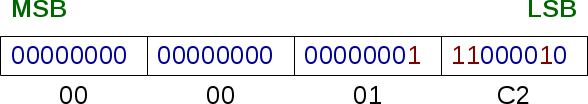
\includegraphics[width=0.9\textwidth]{imgs/big_endian.png}}
    \vfill
    \uncover<3->{Little Endian (más común):}
    \visible<3->{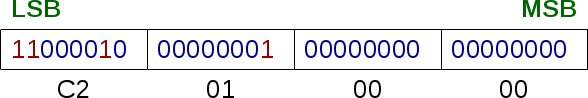
\includegraphics[width=0.9\textwidth]{imgs/little_endian.png}}
\end{frame}

\subsection{Investigando un juego}
\begin{frame}{Tinke}
    \only<1>{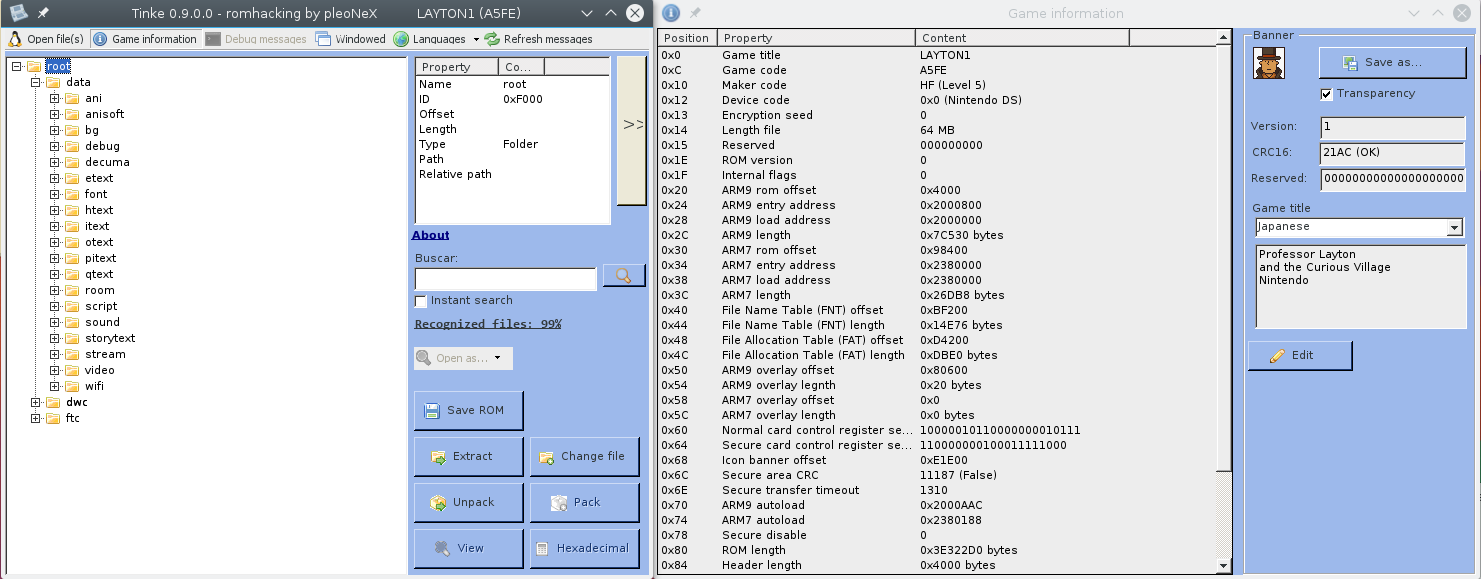
\includegraphics[width=\textwidth]{imgs/tinke.png}}
    \only<2>{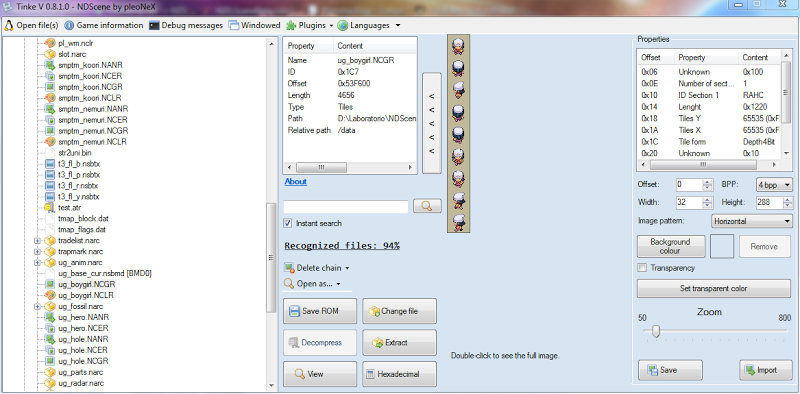
\includegraphics[width=\textwidth]{imgs/tinke_preview.png}}
\end{frame}

\begin{frame}{Tipos de ficheros}
    \begin{columns}
    \begin{column}{0.5\textwidth}
        \begin{itemize}
            \item 
\includegraphics{imgs/palette.png}~Paleta
            \item 
\includegraphics{imgs/picture.png}~Tiles
            \item 
\includegraphics{imgs/picture_link.png}~Map
            \item 
\includegraphics{imgs/pictures.png}~Sprites
            \item 
\includegraphics{imgs/picture_go.png}~Animaciones
            \item 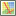
\includegraphics{imgs/map.png}~Modelos 3D
            \item 
\includegraphics{imgs/image.png}~Texturas
            \item 
\includegraphics{imgs/photo.png}~Imagen completa
        \end{itemize}
    \end{column}
    \hfill
    \begin{column}{0.5\textwidth}
        \begin{itemize}
            \item 
\includegraphics{imgs/page_white_text.png}~Texto
            \item 
\includegraphics{imgs/font.png}~Tipografía
            \item 
\includegraphics{imgs/script.png}~Scripts
            \item 
\includegraphics{imgs/compress.png}~Archivo comprimido
            \item 
\includegraphics{imgs/package.png}~Paquete
            \item 
\includegraphics{imgs/music.png}~Música
            \item 
\includegraphics{imgs/film.png}~Vídeo
        \end{itemize}
    \end{column}
    \end{columns}
\end{frame}

\subsection{Editar juegos}
\begin{frame}{Modificando textos}
    \begin{columns}
    \begin{column}{0.5\textwidth}
        \begin{enumerate}
            \item<1-> Localizar texto a modificar
            \item<2-> Abrir juego en Tinke
            \item<3-> Localizar textos
            \item<4-> Extraer archivo
            \item<5-> Modificar con editor
            \item<6-> Importar archivo
            \item<7-> Generar ROM
            \item<8-> Probar en DeSmuME
        \end{enumerate}
    \end{column}
    \hfill
    \begin{column}{0.5\textwidth}
        \centering
        \only<1>{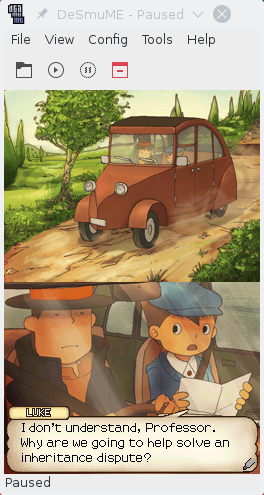
\includegraphics[width=0.7\textwidth]{imgs/mod1.png}}
        \only<2>{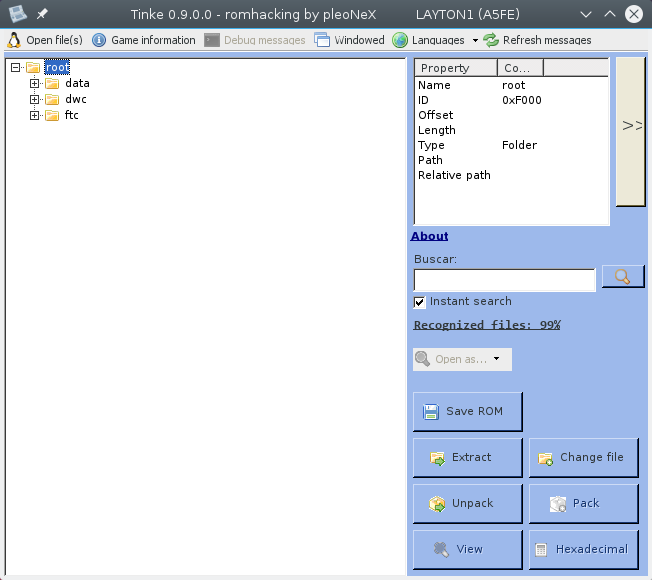
\includegraphics[width=\textwidth]{imgs/mod2.png}}
        \only<3>{\includegraphics[width=\textwidth]{imgs/mod3.png}}
        \only<4>{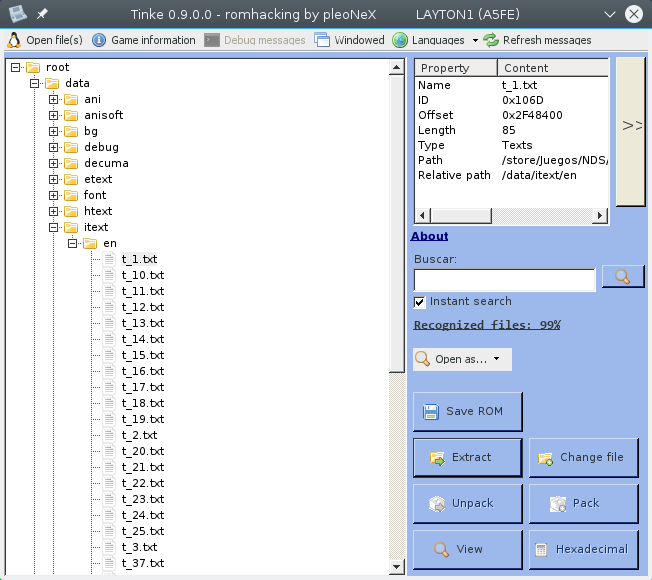
\includegraphics[width=\textwidth]{imgs/mod4.png}}
        \only<5>{\includegraphics[width=\textwidth]{imgs/mod5.png}}
        \only<6>{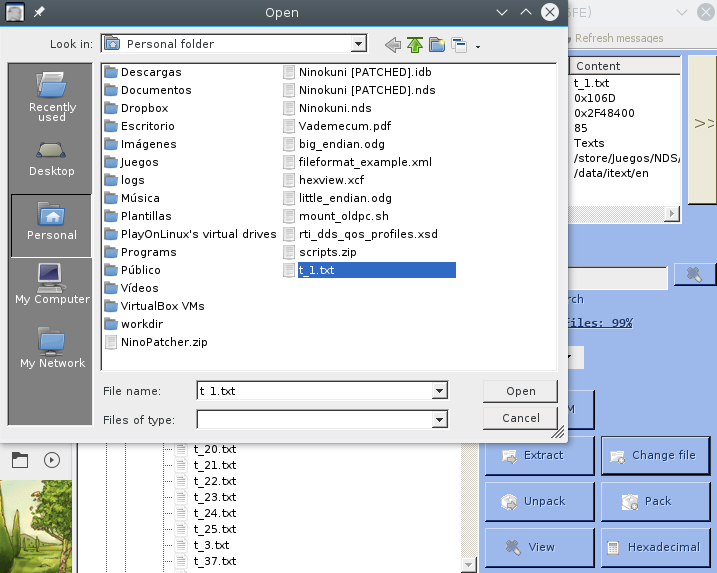
\includegraphics[width=\textwidth]{imgs/mod6.png}}
        \only<7>{\includegraphics[width=\textwidth]{imgs/mod7.png}}
        \only<8>{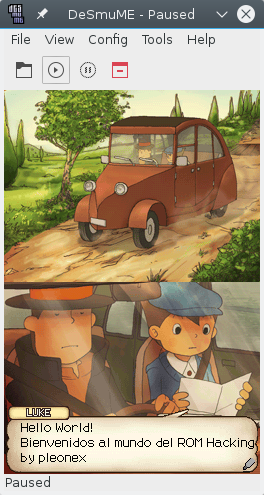
\includegraphics[width=0.7\textwidth]{imgs/mod8.png}}
        \only<9>{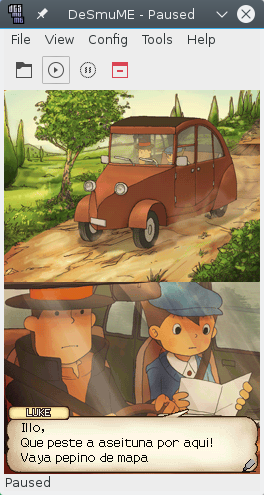
\includegraphics[width=0.7\textwidth]{imgs/pepino.png}}
    \end{column}
    \end{columns}
\end{frame}

\subsection{Publicar cambios}
\begin{frame}{Parches}
    \begin{columns}
    \begin{column}{0.6\textwidth}
        \small
        \begin{wideitemize}
            \item<1-> Solo contienen las modificaciones
            \item<2-> \textbf{No subir el juego modificado}
            \item<3-> Tamaño pequeño (entre 1 y 20 MB)
            \item<4-> Formatos comunes: IPS y xDelta
        \end{wideitemize}
    \end{column}
    \begin{column}{0.4\textwidth}
        \includegraphics[width=\textwidth]{imgs/ninopatcher.png}
    \end{column}
    \end{columns}
\end{frame}

\begin{frame}{xDelta}
    \begin{columns}
    \begin{column}{0.7\textwidth}
        \footnotesize
        \begin{wideitemize}
            \item<1-> Windows: xdelta UI \\ \url{http://www.romhacking.net/utilities/598/}

            \item<2-> Mac OS X: Multipatch \\ \url{http://projects.sappharad.com/tools/multipatch.html}

            \item<3-> Linux: xdelta
            \begin{itemize}
                \footnotesize
                \item Parchear: \\ \texttt{xdelta -d -s ORIGINAL PARCHE}
                \item Crear parche: \\ \texttt{xdelta -9 -s ORIGINAL MODIFICADO PARCHE}
            \end{itemize}
        \end{wideitemize}
    \end{column}
    \begin{column}{0.3\textwidth}
        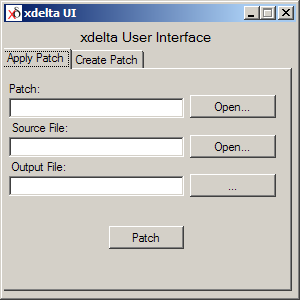
\includegraphics[width=\textwidth]{imgs/xdelta_windows.png}
        \vfill
        \visible<2->{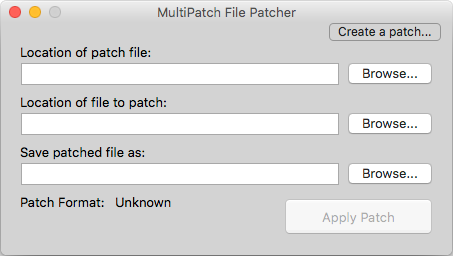
\includegraphics[width=\textwidth]{imgs/xdelta_mac.png}}
    \end{column}
    \end{columns}
\end{frame}

\section{Programas de edición}
\subsection{Pokémon}
\begin{frame}{Advanced Map}
    \centering
    \includegraphics[width=\textwidth]{imgs/advanced_map.png} \\
    Proyecto: \url{http://ampage.no-ip.info/}
\end{frame}

\begin{frame}{Spiky's DS Map Editor}
    \centering
    \includegraphics[width=0.85\textwidth]{imgs/sdme.png} \\
    Proyecto: \url{https://github.com/MarcRiera/SDSME}
\end{frame}

\subsection{New Super Mario Bros DS}
\begin{frame}{NSMB Editor}
    \centering
    \includegraphics[width=\textwidth]{imgs/nsmbe.png} \\
    Proyecto: \url{https://github.com/Dirbaio/NSMB-Editor}
\end{frame}

\subsection{Super Mario 64 DS}
\begin{frame}{Super Mario 64 Editor}
    \centering
    \includegraphics[width=0.9\textwidth]{imgs/sm64ds.png} \\
    Descarga: \url{http://www.romhacking.net/utilities/764}
\end{frame}

\subsection{Ni no kuni}
\begin{frame}{NinoCompiler}
    \begin{tikzpicture}
        \node<1-> (img1) at (0,0) {\includegraphics[width=\textwidth]{imgs/ninoscritor.png}};

        \node<2-> (img2) at (-1.2, 0.7) {\includegraphics[width=0.75\textwidth]{imgs/ninoxml.png}};
        \node<3-> (img3) at (2,-1) {\includegraphics[width=0.3\textwidth]{imgs/ninoimg.png}\huge\textrightarrow\includegraphics[width=0.3\textwidth]{imgs/ninoimg_trans.png}};
        \node<4-> (img4) at (0,0) {\includegraphics[width=0.5\textwidth]{imgs/ninocompiler.png}};
    \end{tikzpicture}

    \visible<4->{\centering
    Proyecto: \url{http://gradienwords.com} \\
    GitHub: \url{https://github.com/pleonex/Ninokuni}}
\end{frame}

    \section{Reto}
\begin{frame}{Reto}
    \Huge\centering\textbf{CHALLENGE TIME!}
\end{frame}

\subsection{The Legend of Zelda: Phantom Hourglass}
\begin{frame}[t]{Contenido sorpresa}
    \begin{columns}
    \begin{column}[T]{0.5\textwidth}
        \centering
        \visible<2->{¿\textit{/Test/picture.narc}?\\\vspace{5pt}}
        \visible<3->{\includegraphics[width=\textwidth]{imgs/zelda_dog.png}}
    \end{column}
    \hfill
    \begin{column}[T]{0.5\textwidth}
        \centering
        \visible<4->{¿\textit{/Test/BgMap.narc}?\\\vspace{5pt}}
        \visible<5->{\includegraphics[width=0.5\textwidth]{imgs/zelda_batch.png}}
    \end{column}
    \end{columns}
\end{frame}

% La idea es modificar el texto e imagenes de la intro.
\begin{frame}{Historia}
    % 0. Contenido de test
    % 1. Cambiar un texto del medio para hacer calculos de punteros y tener que
    % mover el siguiente.
    % 2. Cambiar imagen con map
    % 3. Poner una ecuacion que fuerce crear caracteres
    % 4. Cambiar el mapa.
\end{frame}


\end{document}
